\chapter{Ενισχυτική Μάθηση}
\label{chap:rl}
\section{Γενικά}

Η Ενισχυτική Μάθηση (ΕΜ) (\en{Reinforcement Learning (RL)}) αποτελεί ένα από τους τρεις κύριους κλάδους της μηχανικής
μάθησης και ασχολείται με το πώς ένα σύστημα, ο πράκτορας (\en{agent}), θα πρέπει να ενεργήσει μέσα σε ένα δυναμικό
περιβάλλον (\en{environment}) ώστε να μεγιστοποιήσει την ανταμοιβή του (\en{reward}) \cite{aigreek}. Ο πράκτορας κινείται μέσα από μια σειρά
καταστάσεων (\en{states}) μέχρι να βρεθεί σε μια προκαθορισμένη τελική κατάσταση\cite{drlmaze}.
Αυτός ο πράκτορας αλληλεπιδρά με το περιβάλλον του, παρατηρεί τις συνέπειες των πράξεών του και
μαθαίνει ποιες κινήσεις είναι επιτυχημένες με βάση κάποια μετρική κέρδους. Για παράδειγμα,
ο πράκτορας θα μπορούσε να είναι ένα ποντίκι το οποίο προσπαθεί να βρει την συντομότερη διαδρομή. ξεκινώντας από
ένα αρχικό κελί και φτάνοντας στο τελικό κελί που έχει το τυρί, μέσα σε ένα λαβύρινθο.

Ο πράκτορας δεν τροφοδοτείται με πληροφορίες σχετικά με το ποιες είναι οι βέλτιστες ενέργειες (\en{actions}),
αλλά πρέπει ο ίδιος να ανακαλύψει ποιες είναι αυτές που προσφέρουν την μέγιστη ανταμοιβή, δοκιμάζοντάς τες \cite{rlbook} και
μαθαίνοντας από τις επιτυχίες και τα λάθη του.
Επιπλέον, σε πολλές περιπτώσεις οι ενέργειες του πράκτορα δεν επηρεάζουν μόνο την άμεση ανταμοιβή που θα πάρει,
αλλά και την ανταμοιβή στην επόμενη κατάσταση, και πιθανώς όλες τις επόμενες ανταμοιβές. Έτσι, μπορεί να υπάρξουν
καταστάσεις που ο πράκτορας θα πρέπει να θυσιάσει την άμεση ανταμοιβή για να αποκτήσει καλύτερες ανταμοιβές μακροπρόθεσμα.
Έτσι, βασικά στοιχεία της ΕΜ είναι η χρήση τεχνικών \textit{δοκιμής-και-λάθους \en{(trial-and-error)}} μέσα σε περιβάλλοντα
που οι αμοιβές μπορεί να είναι \textit{καθυστερημένες}.

Μια κομβική ιδέα, πάνω στην οποία στηρίζεται η ΕΜ, είναι η υπόθεση της ανταμοιβής (\en{reward hypothesis}), δηλαδή η ιδέα
ότι κάθε στόχος μπορεί να εκφραστεί σαν την μεγιστοποίηση ενός σήματος ανταμοιβής. Πιο φορμαλιστικά, η κάθε στόχος
μπορεί να εκφραστεί ως η μεγιστοποίηση της αναμενόμενης αξίας του σωρευτικού (\en{cummulative}) αθροίσματος ενός μονοδιάστατου
σήματος \cite{rlbook}. Η ιδέα αυτή δεν περιορίζεται μόνο στο πεδίο της ΕΜ, αλλά μπορεί να χρησιμοποιηθεί για την επεξήγηση βιολογικών
και άλλων φυσιολογικών συστημάτων.
Επιπλέον, η ανταμοιβή αυτή δεν χρειάζεται απαραίτητα να είναι θετικός αριθμός, αλλά ακόμα και όταν παίρνει αρνητικές τιμές, συνεχίζουμε να την καλούμε
με τον όρο ανταμοιβή. Συνεχίζοντας το προηγούμενο παράδειγμα με τον λαβύρινθο, η ανταμοιβή μπορεί να είναι αρνητική σε κάθε βήμα του ποντικού
μέχρι την έξοδο, υπό την έννοια ότι μειώνεται το τυρί που θα λάβει ανάλογα τον χρόνο που θα κάνει να βγει από τον λαβύρινθο.
Τότε, ο στόχος τελικά είναι η ελαχιστοποίηση της απόλυτης τιμής της ανταμοιβής, δηλαδή η έξοδος στα λιγότερα βήματα.

Το πεδίο της ΕΜ έχει τις ρίζες του σε δύο ερευνητικές περιοχές. Η πρώτη είναι η συμπεριφορική ψυχολογία, από όπου προέρχεται το
παράδειγμα της δοκιμής-και-λάθους, και η δεύτερη είναι η περιοχή του βέλτιστου ελέγχου, από όπου η ΕΜ δανείζεται
τον μαθηματικό φορμαλισμό, και κυρίως την τεχνική του δυναμικού προγραμματισμού που υποστηρίζει το πεδίο. Είναι σημαντικό να γνωρίζουμε ότι η ΕΜ
βρίσκεται στην τομή πολλών διαφορετικών επιστημονικών πεδίων, όπως φαίνεται στο Σχήμα~\ref{fig:faces_rl}\cite{silver2015}.
Όλα αυτά τα πεδία προσεγγίζουν ένα παρόμοιο πρόβλημα, αλλά απο διαφορετική σκοπιά και με διαφορετικές παραμέτρους.

\begin{figure}
    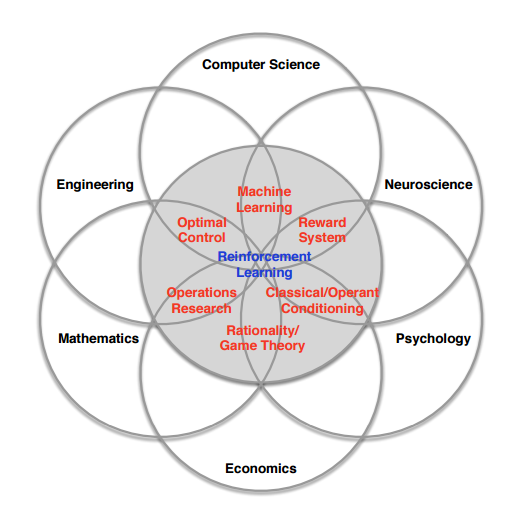
\includegraphics[width=0.8\textwidth]{body_matter/reinforcement_learning/images/faces_of_rl.png}
    \Centering
    \caption{Τα επιστημονικά πεδία που σχετίζονται με την ενισχυτική μάθηση \cite{silver2015}}
    \label{fig:faces_rl}
\end{figure}

Είναι σημαντικό να γνωρίζουμε πώς η ΕΜ συγκρίνεται με τις άλλες τεχνικές μηχανικής μάθησης,
την επιβλεπόμενη (\en{supervised learning}) και τη μη επιβλεπόμενη μάθηση \en{(unsupervised learning)}, καθώς
έχουν σημαντικές διαφορές.

Η κύρια διαφορά μεταξύ της επιβλεπόμενης μάθησης και της ΕΜ είναι ότι στην επιβλεπόμενη
μάθηση, το μοντέλο εκπαιδεύεται πάνω σε δείγματα (\en{samples}) και ετικέτες (\en{labels}), και κάθε πρόβλεψη θεωρείται
μοναδικό γεγονός. Στόχος είναι η προσέγγιση μιας άγνωστης συνάρτησης με βάση τα δεδομένα.
Αντίθετα, στην ΕΜ, μπορούν να υπάρχουν πολλά βήματα πριν ο πράκτορας μάθει αν η απόφαση που πήρε ήταν
σωστή, και είναι πιθανό να μην μάθει ποτέ ποια ήταν η αληθής/βέλτιστη τιμή. Το μόνο που παρατηρεί είναι η
επίδραση που είχαν οι πράξεις του στο περιβάλλον.

Όσον αφορά τη μη επιβλεπόμενη μάθηση, μπορεί σε μια πρώτη ματιά να φαίνεται παρόμοια με την ΕΜ, ωστόσο στόχος της
είναι η εύρεση κρυμμένης δομής σε δεδομένα τα οποία δεν έχουν ετικέτες. Η ΕΜ έχει διαφορετικό στόχο, ο οποίος είναι η
μεγιστοποίηση του σήματος ανταμοιβής. Παρόλο που η εύρεση δομής είναι πολύ σημαντική και στην ΕΜ ώστε να μπορέσει ο πράκτορας
να επιλέξει τις κατάλληλες κινήσεις, η εύρεση αυτή από μόνη της δεν επιτυγχάνει τον στόχο της ΕΜ.

Ένα από τα κύρια προβλήματα της ΕΜ, που δεν συναντάται στις άλλες μορφές μηχανικής μάθησης, είναι
ο συμβιβασμός μεταξύ \textit{εξερεύνησης και εκμετάλλευσης}. Για να μεγιστοποιήσει ο πράκτορας την ανταμοιβή του,
θα προτιμήσει τις ενέργειες που δοκίμασε στο παρελθόν και του προσέφεραν μεγάλη ανταμοιβή. Αλλά
για να ανακαλύψει τέτοιες ενέργειες, θα πρέπει να δοκιμάσει ενέργειες που δεν έχει δοκιμάσει στο παρελθόν.
Έτσι, ο πράκτορας πρέπει να \textit{εκμεταλλευτεί} το τι έχει ήδη βιώσει ώστε να αποκτήσει μεγάλες ανταμοιβές,
αλλά πρέπει και να \textit{εξερευνήσει}, ώστε να πάρει καλύτερες αποφάσεις στο μέλλον. Το δίλημμα λοιπόν γίνεται
το ποια από τις δύο στρατηγικές να επιλέξει κάθε φορά, καθώς καμία δεν μπορεί εφαρμοστεί αποκλειστικά για
να επιτευχθεί ο στόχος του πράκτορα. Ως αποτέλεσμα, ο πράκτορας πρέπει να δοκιμάσει διάφορες
κινήσεις και προοδευτικά να προτιμήσει αυτές που θεωρεί καλύτερες. Καθώς πολλά από τα προβλήματα που
θέλουμε να λύσουμε με ΕΜ είναι \textit{στοχαστικά}, ο πράκτορας πρέπει να δοκιμάσει κάθε πράξη πολλές φορές
για να πάρει μια αξιόπιστη εκτίμηση της προσδοκώμενης ανταμοιβής.


\section{Στοιχεία της ΕΜ}

Πέρα από τον πράκτορα και το περιβάλλον, υπάρχουν ακόμα τέσσερα κύρια στοιχεία τα οποία όλα μαζί αποτελούν
ένα σύστημα ΕΜ. Αυτά είναι:
\begin{itemize}
    \item Η πολιτική (\en{policy}), η οποία ορίζει την συμπεριφορά του πράκτορα για μια δοθείσα
          χρονική στιγμή. Ειδικότερα, η πολιτική είναι μια αντιστοίχιση των καταστάσεων
          που αντιλαμβάνεται ο πράκτορας με τις ενέργειες που κάνει σε αυτές τις καταστάσεις (πιο συγκεκριμένα στις πιθανότητες αυτών των ενεργειών). Οι
          πολιτικές μπορεί να είναι και στοχαστικές, προσδιορίζοντας μια πιθανότητα για κάθε ενέργεια.
    \item Το σήμα ανταμοιβής, το οποίο αναφέρθηκε και νωρίτερα. Το σήμα αυτό προσδιορίζει τον στόχο ενός προβλήματος
          ΕΜ. Σε κάθε χρονικό βήμα, το περιβάλλον στέλνει στον πράκτορα έναν αριθμό, την ανταμοιβή για την συγκεκριμένη χρονική στιγμή.
          Ο μόνος στόχος του πράκτορα είναι να μεγιστοποιήσει την συνολική ανταμοιβή που λαμβάνει
          μακροπρόθεσμα. Έτσι το σήμα της ανταμοιβής προσδιορίζει ποια είναι τα θετικά και τα αρνητικά
          γεγονότα για τον πράκτορα. Είναι σημαντικό η ανταμοιβή να προσδιορίζει ακριβώς το
          τι θέλουμε να πετύχουμε, όμως δεν πρέπει να περιέχει πληροφορίες για το πώς θα πετύχουμε τον στόχο αυτό.
          Αυτές οι πληροφορίες μπορούν να τοποθετηθούν μέσα στην πολιτική ή στην συνάρτηση αξίας, η οποία περιγράφεται παρακάτω.
          Το σήμα είναι η κύρια βάση μέσω της οποίας αλλάζει η πολιτική.
          Για παράδειγμα, αν ο πράκτορας επιλέξει μια ενέργεια με μικρή ανταμοιβή, στην περίπτωση που υπάρξει η ίδια κατάσταση στο μέλλον,
          η πολιτική του ίσως να αλλάξει για να επιλέξει μια άλλη ενέργεια που ίσως έχει μεγαλύτερη ανταμοιβή. Γενικά, οι
          ανταμοιβές μπορεί να είναι στοχαστικές συναρτήσεις της κατάστασης του περιβάλλοντος και των
          ενεργειών που επιλέχθηκαν.
    \item Η συνάρτηση αξίας κάθε κατάστασης \en{(value function)}. Αντίθετα από το σήμα
          ανταμοιβής που μας επιστρέφει το τί είναι καλό άμεσα, η συνάρτηση αξίας προσδιορίζει το τι είναι καλό μακροπρόθεσμα.
          Σε γενικές γραμμές, η αξία μιας κατάστασης είναι η συνολική ανταμοιβή που δύναται
          να αποκτήσει ένας πράκτορας στο μέλλον, ξεκινώντας από την συγκεκριμένη κατάσταση. Έτσι,
          ενώ οι ανταμοιβές προσδιορίζουν την άμεση και εσωτερική ελκυστικότητα των καταστάσεων του περιβάλλοντος,
          η αξία υποδεικνύει την μακροπρόθεσμη ελκυστικότητα των καταστάσεων, λαμβάνοντας υπόψιν τις καταστάσεις
          που θα ακολουθήσουν και τις διαθέσιμες ανταμοιβές σε αυτές. Συνεπώς, μια κατάσταση
          με χαμηλή ανταμοιβή, μπορεί να έχει μεγάλη αξία γιατί οδηγεί σε καταστάσεις με μεγαλύτερες ανταμοιβές.
          Συμπερασματικά, η συνάρτηση αξίας προσδιορίζει πόσο καλό είναι για ένα πράκτορα να είναι στην συγκεκριμένη κατάσταση.
    \item Προαιρετικά, ένα μοντέλο του περιβάλλοντος (\en{model}). Το μοντέλο ενός συστήματος ΕΜ μιμείται τη
          συμπεριφορά του περιβάλλοντος, ή πιο γενικά, επιτρέπει τη δημιουργία συμπερασμάτων για το πώς θα
          συμπεριφερθεί το περιβάλλον. Τα μοντέλα χρησιμοποιούνται για σχεδιασμό \en{(planning)}, δηλαδή την επιλογή της
          σειράς των δράσεων λαμβάνοντας υπόψιν πιθανές μελλοντικές καταστάσεις, πριν τις βιώσει ο πράκτορας.
          Μέθοδοι επίλυσης προβλημάτων ΕΜ που χρησιμοποιούν μοντέλα και σχεδιασμό λέγονται μέθοδοι βασισμένοι
          σε μοντέλα (\en{model-based}). Αν οι μέθοδοι επίλυσης δεν βασίζονται σε κάποιο μοντέλο, δηλαδή μαθαίνουν ρητά μέσω
          δοκιμής-και-λάθους, λέγονται μέθοδοι χωρίς μοντέλο (\en{model-free}).
\end{itemize}

Πιο φορμαλιστικά, σε ένα περιβάλλον ΕΜ, ένας αυτόνομος πράκτορας, ελεγχόμενος από ένα αλγόριθμο μηχανικής μάθησης,
παρατηρεί μια κατάσταση $s_t$ από το περιβάλλον του σε ένα χρονικό βήμα $t$. Οι χρονικές στιγμές στην περιγραφή αυτή είναι διακριτές,
δηλαδή $t=0,1,2,\ldots$, αλλά θα μπορούσαν να είναι και συνεχείς, χωρίς μεγάλες διαφορές. Οι καταστάσεις προέρχονται από τον
χώρο καταστάσεων $\mathcal{S}$. Ο πράκτορας αλληλεπιδρά με το περιβάλλον επιλέγοντας μια ενέργεια $a_t$ με βάση την κατάσταση
$s_t$, επιλεγμένη από ένα χώρο ενεργειών $\mathcal{A}(s)$. Όταν ο πράκτορας εκτελέσει την ενέργεια, τότε το περιβάλλον,
μεταβαίνει σε μια νέα κατάσταση $s_{t+1}$, με βάση την τρέχουσα κατάσταση και την επιλεγμένη
ενέργεια \cite{drlbs}. Σε κάθε τριπλέτα (κατάστασης, ενέργειας, νέας κατάστασης), αντιστοιχεί μια πιθανότητα μετάβασης
$p(\{S_{t+1}=s'|S_t=s, A_{t}=a\})$. Σε κάθε κατάσταση, ο πράκτορας μπορεί είτε να παρατηρήσει την πλήρη δυναμική του
περιβάλλοντος είτε μέρος αυτού. Ο πράκτορας επίσης, λαμβάνει και μια μονοδιάστατη ανταμοιβή $R_t$,
η οποία προέρχεται από την τριπλέτα (κατάστασης, ενέργειας, νέας κατάστασης), και συμβολίζεται ως
$R(s_{t-1}, a_{t-1}, s_t)$. Αυτή η ανταμοιβή δεν είναι γνωστή αρχικά στον πράκτορα και
δρα ως μια μορφή ανατροφοδότησης για τις δράσεις του.
Αυτή η διαδικασία αναπαριστάται οπτικά στο Σχήμα~\ref{fig:agent_environment}.


Συνήθως, ο πράκτορας διατηρεί μια εσωτερική κατάσταση, η οποία περιλαμβάνει κομμάτια της κατάστασης του περιβάλλοντος τα οποία θεωρούνται
σημαντικά, καθώς και άλλες πληροφορίες που αξιολογούνται ως σημαντικές. Σε αυτή την εσωτερική κατάσταση, ο πράκτορας
διατηρεί μια αντιστοίχιση μεταξύ κατάστασης και ενέργειας, η οποία συμβολίζεται ως $p(a_t | s_t)$.

\begin{figure}[ht]
    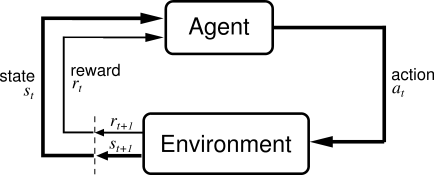
\includegraphics[width=0.8\textwidth]{body_matter/reinforcement_learning/images/agent_environment.png}
    \Centering
    \caption{Αλληλεπίδραση πράκτορα και περιβάλλοντος}
    \label{fig:agent_environment}
\end{figure}


Η βέλτιστη σειρά ενεργειών προσδιορίζεται από τις ανταμοιβές που παρέχει το περιβάλλον. Ο τελικός στόχος του πράκτορα είναι να μάθει μια
πολιτική $π$, η οποία μεγιστοποιεί την αναμενόμενη απόδοση (σωρευτική, ανταμοιβή με έκπτωση \en{(discounted reward)}). Δοθείσας μιας κατάστασης
η πολιτική αποφασίζει την επόμενη ενέργεια την οποία θα κάνει ο πράκτορας. Μια βέλτιστη πολιτική είναι η πολιτική η οποία μεγιστοποιεί
την αναμενόμενη απόδοση στο συγκεκριμένο περιβάλλον.


\subsection{Παρατηρησιμότητα}

Πέρα απο την περιγραφή του συστήματος ΕΜ με βάση την ύπαρξη ή όχι μοντέλου του περιβάλλοντος, ένας
άλλος τρόπος να περιγράψουμε τα συστήματα ΕΜ είναι με βάση το περιβάλλον στο οποίο βρίσκονται οι πράκτορες.
Η πρώτη περίπτωση είναι να είναι αυτό το περιβάλλον πλήρως παρατηρήσιμο, δηλαδή ο πράκτορας μπορεί να παρατηρήσει κάθε πληροφορία για την δυναμική του περιβάλλοντος.
Αυτό φυσικά δεν σημαίνει ότι κάθε παρατήρηση θα είναι χρήσιμη. Συνεπώς, η κατάσταση του πράκτορα θα είναι το υποσύνολο των παρατηρήσεων που είναι χρήσιμες.
Αυτά τα περιβάλλοντα ικανοποιούν την Μαρκοβιανή ιδιότητα, δηλαδή η επόμενη κατάσταση (και κατά βάση όλες οι επόμενες καταστάσεις) εξαρτάται μόνο από
την τρέχουσα κατάσταση και όχι αθροιστικά από τις προηγούμενες. Όταν ισχύει αυτή η ιδιότητα, τότε μπορούμε να μοντελοποιήσουμε το πρόβλημα ως μια
Μαρκοβιανή Διαδικασία Αποφάσεων (\en{Markov Decision Process}). Η δεύτερη περίπτωση, αφορά περιβάλλοντα που δεν είναι πλήρως
παρατηρήσιμα. Για παράδειγμα, στην περίπτωση που ένα ρομπότ κινείται μέσα σε ένα δωμάτιο. Καθώς το περιβάλλον του δωματίου περιγράφεται
από πολλές παραμέτρους, οι οποίες δεν είναι όλες γνωστές - για παράδειγμα μέσα στο δωμάτιο μπορεί να κινείται και μια γάτα,
το ρομπότ δεν γίνεται σε κάθε κίνησή του να γνωρίζει τα πάντα.

Η Μαρκοβιανή ιδιότητα ορίζεται ως:
\begin{equation}
    p(r,s | \mathcal{H}_t, A_t) = p(r,s|S_t, A_t)
\end{equation}

το οποίο σημαίνει ότι η πιθανότητα να βρεθούμε στην κατάσταση $s$ με ανταμοιβή $r$, αν γνωρίζουμε
ολόκληρη την ιστορία της αλληλεπίδρασης του πράκτορα με το περιβάλλον ($\mathcal{H}$), κάνοντας
την ενέργεια $A_t$ (αριστερό μέρος) είναι ίδια με την πιθανότητα να βρεθούμε στην κατάσταση $s$ με
ανταμοιβή $r$ γνωρίζοντας μόνο την τελευταία κατάσταση $S_t$ στην οποία βρισκόταν ο πράκτορας
και την ενέργεια $A_t$ που έκανε (δεξί μέρος).

\section{Μαρκοβιανές Διαδικασίες Αποφάσεων (ΜΔΑ)}

Για την καλύτερη κατανόηση της ΕΜ, είναι χρήσιμο να περιορίσουμε το πρόβλημα σε μορφή που είναι μια ΜΔΑ.
Συγκεκριμένα, σε διακριτό χρόνο, η αρχή της πορείας ενός πράκτορα θα είναι

\begin{equation*}
    S_0, A_0, R_1, S_1, A_1, R_2, S_2, A_2,\ldots
\end{equation*}

Σε μια πεπερασμένη ΜΔΑ, οι καταστάσεις, οι ενέργειες και οι ανταμοιβές είναι τα σύνολα
($\mathcal{S}, \mathcal{A}, \mathcal{R}$) με πεπερασμένο αριθμό στοιχείων.
Σε αυτή την περίπτωση οι τυχαίες μεταβλητές $R_t$ και $S_t$ έχουν μια καλά ορισμένη διακριτή πιθανότητα,
η οποία εξαρτάται μόνο από την προηγούμενη κατάσταση $S_{t-1}$ και ενέργεια $A_{t-1}$.
Έτσι η δυναμική της ΜΔΑ ορίζεται από τη συνάρτηση, η οποία λόγω της Μαρκοβιανής ιδιότητας προσδιορίζει πλήρως την δυναμική του συστήματος.


\begin{equation}
    p(s', r | s, a) = p(S_t = s', R_t = r | S_{t-1} = s, A_{t-1} = a)
\end{equation}

Όσον αφορά το σήμα ανταμοιβής, ο στόχος είναι η μεγιστοποίησή του σε βάθος χρόνου.
Αυτό αναφέρεται στη βιβλιογραφία ως απόδοση (\en{return}), η οποία πολύ συχνά αναπαριστάται ως $G_t$.

Ανάλογα με το αν τερματίζει ένα πρόβλημα, αυτό μπορεί να θεωρηθεί επεισοδιακό ή συνεχές. Σε ένα επεισοδιακό πρόβλημα,
υπάρχει πάντα μια τελική κατάσταση (π.χ., η έξοδος ενός λαβυρίνθου).
Σε ένα συνεχές πρόβλημα, δεν υπάρχει αυτός ο διαχωρισμός σε επεισόδια, αλλά η αλληλεπίδραση συνεχίζεται ατέρμονα.
Για να μπορέσουμε να υπολογίσουμε την απόδοση ακόμα και σε συνεχή προβλήματα, συνήθως την ορίζουμε ως

\begin{equation}
    G_t = R_{t+1} + γ R_{t+2} + γ^2 R_{t+3} + \ldots = \sum_{k=0}^{\infty}γ^k R_{t+k+1}
\end{equation}

όπου $ 0 \leq γ \leq 1$ είναι μια παράμετρος η οποία ονομάζεται παράγοντας έκπτωσης.
Ο παράγοντας αυτός επηρεάζει το πόσο σημασία έχουν οι μετέπειτα ανταμοιβές.
Επίσης, έχει μαθηματική αξία, καθώς εξασφαλίζει ότι η απόδοση είναι πάντα φραγμένη (για $γ < 1$).

Για $γ = 0$, ο πράκτορας είναι μυωπικός, δηλαδή ενδιαφέρεται να εξασφαλίσει την καλύτερη ανταμοιβή σε κάθε βήμα,
ανεξάρτητα αν αυτό σημαίνει ότι θα χάσει καλύτερες ανταμοιβές αργότερα, ενώ όσο η τιμή πηγαίνει προς το 1,
ο πράκτορας βλέπει όλο και πιο μακριά.

Με βάση τα παραπάνω, μπορούμε πλέον να προσδιορίσουμε και πιο φορμαλιστικά την περιγραφή της πολιτικής του πράκτορα και της συνάρτησης αξίας.
Όπως αναφέρθηκε ήδη η πολιτική είναι μια αντιστοίχηση μεταξύ καταστάσεων και πιθανοτήτων επιλογής πράξεων.
Αν ένας πράκτορας ακολουθεί μια πολιτική $π$ την χρονική στιγμή $t$,
τότε $π(a|s)$ είναι η πιθανότητα να επιλεχθεί $A_t = a$, αν $S_t =s$.

Η συνάρτηση αξίας μιας κατάστασης $s$ όταν ο πράκτορας ακολουθεί μια πολιτική $π$,
με ένδειξη $υ_π(s)$ είναι η αναμενόμενη απόδοση όταν ο πράκτορας ξεκινήσει από την κατάσταση $s$
και ακολουθήσει την πολιτική $π$. Για ΜΔΑ, αυτή ορίζεται ως

\begin{equation}
    υ_π(s) = \mathbb{E}_π[G_t\;|\;S_t = s] = \mathbb{E}_π \left[ \sum_{k=0}^{\infty}γ^kR_{t+k+1}\;\bigg|\;S_t = s\right]
\end{equation}

για όλες τις καταστάσεις $s$ του συνόλου $\mathcal{S}$.
Το $\mathbb{E}_π[\cdot]$ είναι η αναμενόμενη τιμή μιας τυχαίας μεταβλητής δεδομένου ότι ο πράκτορας ακολουθεί πολιτική
$π$ και $t$ είναι το χρονικό βήμα. Αυτή η συνάρτηση παραπάνω ορίζεται ως συνάρτηση αξίας-κατάστασης για την πολιτική $π$.

Μπορούμε να ορίσουμε και την συνάρτηση αξίας-ενέργειας για την πολιτική $π$, η οποία ορίζεται ως

\begin{equation}
    q_π(s,a) = \mathbb{E}_π[G_t | S_t = s, A_t = a] = \mathbb{E}_π\left[ \sum_{k=0}^{\infty} γ^k R_{t+k+1} \bigg| S_t = s, A_t = a\right]
\end{equation}

η οποία προσδιορίζει την αξία του να κάνει ο πράκτορας της ενέργεια $a$ στην κατάσταση $s$ υπό την πολιτική $π$,
η οποία είναι η αναμενόμενη απόδοση που θα έχει ο πράκτορας αν στην κατάσταση $s$ κάνει την ενέργεια $a$ και μετά συνεχίσει με την πολιτική $π$.

Οι δύο συναρτήσεις αξίας, μπορούν να υπολογιστούν με βάση την εμπειρία που αποκτά ο πράκτορας κατά την μετάβαση του μεταξύ των καταστάσεων.
Για παράδειγμα αν ακολουθεί την πολιτική $π$, τότε για κάθε κατάσταση, όσο πιο συχνά την επισκέπτεται, τόσο πιο κοντά θα φτάνει η μέση τιμή
στην πραγματική αξία $υ_π(s)$ της κατάστασης. Αντίστοιχα αν κρατάει μέσους όρους για κάθε πράξη σε κάθε κατάσταση, θα φτάσει στην πραγματική
αξία $q_π(s,a)$ της ενέργειας. Οι τεχνικές αυτές ονομάζονται Μόντε Κάρλο (\en{Monte Carlo}), γιατί βρίσκουν μέσους όρους πολλών τυχαίων δειγμάτων πραγματικών αποδόσεων.
Ένας άλλος τρόπος είναι με χρήση συναρτήσεων που προσομοιώνουν τις συναρτήσεις αξιών, και είναι χρήσιμες όταν υπάρχει πολύ μεγάλος αριθμός καταστάσεων
και η αποθήκευση όλων των τιμών δεν είναι δυνατή.

Στόχος της ΕΜ είναι η εύρεση βέλτιστων πολιτικών που θα επιφέρουν μεγάλη ανταμοιβή μακροπρόθεσμα. Έτσι, σε μια ΜΔΑ θέλουμε να δημιουργήσουμε
μια εκτίμηση της βέλτιστης αξίας κάθε ενέργειας $α$ σε κάθε κατάσταση $s$ ($q_*(s,α)$) ή μια εκτίμηση της αξίας κάθε κατάστασης δεδομένης
μιας βέλτιστης επιλογής ενεργειών ($u_*(s)$).

Σε πεπερασμένες ΜΔΑ η βέλτιστη απόφαση είναι πλήρως ορισμένη, και είναι η πολιτική που επιφέρει μεγαλύτερη ή ίση αξία με όλες τις υπόλοιπες πολιτικές.
Αυτή η βέλτιστη πολιτική, δεν είναι δυνατόν να βρεθεί σε πραγματικά προβλήματα, γιατί
\begin{enumerate}
    \item η δυναμική του περιβάλλοντος δεν είναι πλήρως γνωστή,
    \item δεν είναι υπολογιστικά εφικτό να βρεθεί η βέλτιστη πολιτική, πχ γιατί ο χώρος καταστάσεων είναι τεράστιος,
    \item οι καταστάσεις δεν έχουν την Μαρκοβιανή ιδιότητα.
\end{enumerate}

Σε αυτές τις περιπτώσεις, η μόνη μας επιλογή είναι είτε να δημιουργήσουμε προσεγγίσεις της βέλτιστης πολιτικής, να χρησιμοποιήσουμε ευριστικές, ή και τα δύο.

\section{Συμπεράσματα}

Το πρόβλημα της Ενισχυτικής Μάθησης μελετάει την εύρεση βέλτιστων πολιτικών για πράκτορες που κινούνται μέσα σε ένα περιβάλλον,
πολιτικών δηλαδή που προσφέρουν τη μέγιστη αξία στον πράκτορα. Επειδή πολλές φορές η εύρεση της βέλτιστης πολιτικής δεν είναι πρακτικά δυνατή,
χρησιμοποιούμε προσεγγίσεις και ευριστικές.

Στην δική μας εργασία, οι καταστάσεις του περιβάλλοντος είναι γνωστές και πεπερασμένες, αφού είναι φραγμένες από τον αριθμό των θεμάτων που μπορεί
να καταλάβει και συζητήσει ο πράκτορας μας, τα οποία είναι επακριβώς ορισμένα. Επιπλέον, μπορούμε να θεωρήσουμε ότι οι καταστάσεις του διαλόγου
έχουν τη Μαρκοβιανή ιδιότητα, καθώς η τρέχουσα κατάσταση του διαλόγου περιγράφει πλήρως την συζήτηση μέχρι τώρα, αφού περιλαμβάνει όλες τα θέματα που έχουν
αναφερθεί. Το πρόβλημα είναι ότι οι δυναμικές του
συστήματος είναι πλήρως άγνωστες και μεταβλητές, καθώς δεν γνωρίζουμε καμία πληροφορία για τον χρήστη κατά την αρχή της συζήτησης, ώστε να μπορέσουμε
να επιλέξουμε κατάλληλα προτάσεις, και επιπλέον τα ενδιαφέροντα των χρηστών στο σύνολο μετακινούνται με την πάροδο του χρόνου. Επειδή ο συγκεκριμένος
πράκτορας δεν αποκτά πολλές πληροφορίες για το περιβάλλον, καθώς δεν υπάρχουν πολλοί χρήστες, θα πρέπει να απλοποιήσουμε το πρόβλημα και να μην
ασχοληθούμε με το πλήρες πρόβλημα της ενισχυτικής μάθησης, αλλά με ένα πιο περιορισμένο, το πρόβλημα των \en{bandits}.
